%% Uncomment one of these, if you write in English:
%% the 1st when using pdflatex, which directly typesets your document in
%% pdf (use jpg or pdf figures), or
%% the 2nd when producing a ps file (use eps figures, don't use ps figures!).
\documentclass[english,12pt,a4paper,pdftex,elec,utf8]{aaltothesis}
%\documentclass[english,12pt,a4paper,dvips]{aaltothesis}

\usepackage{graphicx}

%% Use this if you write hard core mathematics, these are usually needed
%%
%% Matematiikan fontteja, symboleja ja muotoiluja lisää, näitä tarvitaan usein
\usepackage{amsfonts,amssymb,amsbsy}
\usepackage{epigraph}
%% Use the macros in this package to change how the hyperref package below
%% typesets its hypertext -- hyperlink colour, font, etc. See the package
%% documentation. It also defines the \url macro, so use the package when
%% not using the hyperref package.
%%
%% Jos et jostain syystä pidä, miten alla oleva hyperref-paketti käyttää
%% fontteja, värejä yms., käytä tämän paketin makroja muuttamaan
%% fonttimäärittelyt. Katso paketin dokumentaatiota. Paketti määrittelee
%% \url-makron, joten ota paketti käyttöön, jos et käytä hyperref-pakettia.
%\usepackage{url}

%% Use this if you want to get links and nice output. Works well with pdflatex.
%%
%% Saat pdf-tiedoston viittaukset ja linkit kuntoon seuraavalla paketilla.
%% Paketti toimii erityisen hyvin pdflatexin kanssa.
\usepackage{hyperref}
\hypersetup{pdfpagemode=UseNone, pdfstartview=FitH,
  colorlinks=true,urlcolor=red,linkcolor=blue,citecolor=black,
  pdftitle={A/B Testing, Modify},pdfauthor={Samuli Ulmanen},
  pdfkeywords={abtesting, fremium}}

%% All that is printed on paper starts here
%%
%% Kaikki mikä paperille tulostuu, on tämän jälkeen
\begin{document}

%% Change the school field to specify your school if the automatically
%% set name is wrong
%%
%% Korjaa vastaamaan korkeakouluasi, jos automaattisesti asetettu nimi on
%% virheellinen
% \university{aalto-yliopisto}
% \university{aalto University}
% \school{Sähkötekniikan korkeakoulu}
% \school{School of Electrical Engineering}

%% Only for B.Sc. thesis: Choose your degree programme.
%%
%% Vain kandityölle: Korjaa seuraavat vastaamaan koulutusohjelmaasi
\degreeprogram{Electronics and electrical engineering}
%\degreeprogram{Elektroniikka ja sähkötekniikka}
%%

%% ONLY FOR M.Sc. AND LICENTIATE THESIS: Specify your department,
%% professorship and professorship code.
%%
%% Vain DI/M.Sc.- ja lisensiaatintyölle: valitse laitos,
%% professuuri ja sen professuurikoodi.
\department{Department of Radio Science and Technology}
%\department{Radiotieteen ja -tekniikan laitos}

\professorship{Circuit theory}
%\professorship{Piiriteoria}
\code{S-55}
%%

%% Valitse yksi näistä kolmesta
%%
%% Choose one of these:
%\univdegree{BSc}
\univdegree{MSc}
%\univdegree{Lic}

%% Oma nimi
%%
%% Should be self explanatory...
\author{Samuli Ulmanen}

%% Your thesis title comes here and again before a possible abstract in
%% Finnish or Swedish . If the title is very long and latex does an
%% unsatisfactory job of breaking the lines, you will have to force a
%% linebreak with the \\ control character.
%% Do not hyphenate titles.
%%
%% Opinnäytteen otsikko tulee tähän ja uudelleen englannin- tai
%% ruostinkielisen abstraktin yhteydessä. Älä tavuta otsikkoa ja
%% vältä liian pitkää otsikkotekstiä. Jos latex ryhmittelee otsikon
%% huonosti, voit joutua pakottamaan rivinvaihdon \\ kontrollimerkillä.
%% Muista että otsikkoja ei tavuteta!
%% Jos otsikossa on ja-sana, se ei jää rivin viimeiseksi sanaksi
%% vaan aloittaa uuden rivin.
\thesistitle{Improving Freemium Games with A/B Testing}

\place{Espoo}

%% For B.Sc. thesis use the date when you present your thesis.
%%
%% Kandidaatintyön päivämäärä on sen esityspäivämäärä!
\date{28.2.2014}

%% B.Sc. or M.Sc. thesis supervisor
%% Note the "\" after the comma. This forces the following space to be
%% a normal interword space, not the space that starts a new sentence.
%% This is done because the fullstop isn't the end of the sentence that
%% should be followed by a slightly longer space but is to be followed
%% by a regular space.
%%
%% Kandidaattiseminaarin vastuuopettaja tai diplomityön valvoja.
%% Huomaa tittelissä "\" -merkki pisteen jälkeen,
%% ennen välilyöntiä ja seuraavaa merkkijonoa.
%% Näin tehdään, koska kyseessä ei ole lauseen loppu, jonka jälkeen tulee
%% hieman pidempi väli vaan halutaan tavallinen väli.
\supervisor{Prof.\ Pirjo Professori} %{Prof.\ Pirjo Professori}

%% B.Sc. or M.Sc. thesis advisors(s). You can give upto two advisors in
%% this template. Check with your supervisor how many official advisors
%% you can have.
%%
%% Kandidaatintyön ohjaaja(t) tai diplomityön ohjaaja(t). Ohjaajia saa
%% olla korkeintaan kaksi.
%%
%\advisor{Prof.\ Pirjo Professori}
\advisor{D.Sc.\ (Tech.) Olli Ohjaaja}
%\advisor{M.Sc.\ Polli Pohjaaja}

%% Aalto logo: syntax:
%% Aaltologo: syntaksi:
%%
%% \uselogo{aaltoRed|aaltoBlue|aaltoYellow|aaltoGray|aaltoGrayScale}{?|!|''}
%%
%% Logo language is set to be the same as the document language.
%% Logon kieli on sama kuin dokumentin kieli
%%
\uselogo{aaltoRed}{''}

%% Create the coverpage
%%
%% Tehdään kansilehti
\makecoverpage


%% Note that when writting your master's thesis in English, place
%% the English abstract first followed by the possible Finnish abstract

%% English abstract.
%% All the information required in the abstract (your name, thesis title, etc.)
%% is used as specified above.
%% Specify keywords
%%
%% Kaikki tiivistelmässä tarvittava tieto (nimesi, työnnimi, jne.) käytetään
%% niin kuin se on yllä määritelty.
%% Avainsanat
%%
\keywords{abtesting, freemium}
%% Abstract text
\begin{abstractpage}[english]
  Your abstract in English. Try to keep the abstract short; approximately
  100 words should be enough. The abstract explains your research topic,
  the methods you have used, and the results you obtained.
  Your abstract in English. Try to keep the abstract short; approximately
  100 words should be enough. The abstract explains your research topic,
  the methods you have used, and the results you obtained.

  Your abstract in English. Try to keep the abstract short; approximately
  100 words should be enough. The abstract explains your research topic,
  the methods you have used, and the results you obtained.
  Your abstract in English. Try to keep the abstract short; approximately
  100 words should be enough. The abstract explains your research topic,
  the methods you have used, and the results you obtained.
\end{abstractpage}

%% Force a new page so that the possible English abstract starts on a new page
%%
%% Pakotetaan uusi sivu varmuuden vuoksi, jotta
%% mahdollinen suomenkielinen ja englanninkielinen tiivistelmä
%% eivät tule vahingossakaan samalle sivulle
\newpage

%% Preface
%%
%% Esipuhe
\mysection{Preface}
%\mysection{Esipuhe}
I want to thank Professor Pirjo Professori
and my instructor Olli Ohjaaja for their
good and poor guidance.\\

\vspace{5cm}
Otaniemi, 24.10.2014

\vspace{5mm}
{\hfill Samuli Ulmanen \hspace{1cm}}

%% Force new page after preface
%%
%% Pakotetaan varmuuden vuoksi esipuheen jälkeinen osa
%% alkamaan uudelta sivulta
\newpage


%% Table of contents.
%%
%% Sisällysluettelo
\thesistableofcontents


%% Symbols and abbreviations
%%
%% Symbolit ja lyhenteet
\mysection{Symbols and abbreviations}
%\mysection{Symbolit ja lyhenteet}
\subsection*{Symbols}
%\subsection*{Symbolit}

\begin{tabular}{ll}
%$|a_{ij}|^2$, $|a_i|^2$ & probability of two electrons having momenta
%    $\boldsymbol p_i$ and $\boldsymbol p_j$ ($\boldsymbol p_i$ for $|a_i|^2$) \\
%                 & at any given instant \\
$\mathbf{B}$  & magneettivuon tiheys  \\
$c$              & valon nopeus tyhj\"oss\"a $\approx 3\times10^8$ [m/s]\\
%$p$              & magnitude of momentum \\
%$\boldsymbol p$, $\boldsymbol p_i$, $\boldsymbol p_i^{'}$  & momentum vector \\
%$p$              & magnitude of momentum \\
%$\boldsymbol p$, $\boldsymbol p_i$, $\boldsymbol p_i^{'}$  & momentum vector \\
%$\boldsymbol P$  &  \\
%$p_{\mathrm{F}}$ & Fermi momentum \\
$\omega_{\mathrm{D}}$    & Debye-taajuus \\
$\omega_{\mathrm{latt}}$ & hilan keskim\"a\"ar\"ainen fononitaajuus \\
$\uparrow$       & elektronin spinin suunta yl\"osp\"ain\\
$\downarrow$     & elektronin spinin suunta alasp\"ain
\end{tabular}

\subsection*{Operators}
%\subsection*{Operaattorit}

\begin{tabular}{ll}
$\nabla \times \mathbf{A}$              & vektorin $\mathbf{A}$ roottori\\
$\displaystyle\frac{\mbox{d}}{\mbox{d} t}$ & derivaatta muuttujan $t$ suhteen\\
[3mm]
$\displaystyle\frac{\partial}{\partial t}$  & osittaisderivaatta muuttujan $t$ suhteen \\[3mm]
$\sum_i $                       & Summa indeksin $i$ yli\\
$\mathbf{A} \cdot \mathbf{B}$    & vektorien $\mathbf{A}$ ja $\mathbf{B}$ pistetulo
\end{tabular}

\subsection*{Abbreviations}
%\subsection*{Lyhenteet}

\begin{tabular}{ll}
AC         & vaihtovirta \\
APLAC      & an object-oriented analog circuit simulator and design tool \\
           & (originally Analysis Program for Linear Active Circuits) \\
BCS        & Bardeen-Cooper-Schrieffer \\ %% tavuviiva - nimien v\"aliss\"a
DC         & tasavirta \\
TEM        & transverse eletromagnetic
\end{tabular}


%% Sivulaskurin viilausta opinn\"aytteen vaatimusten mukaan:
%% Aloitetaan sivunumerointi arabialaisilla numeroilla (ja j\"atet\"a\"an
%% leip\"atekstin ensimm\"ainen sivu tyhj\"aksi,
%% ks. alla \thispagestyle{empty}).
%% Pakotetaan lis\"aksi ensimm\"ainen varsinainen tekstisivu alkamaan
%% uudelta sivulta clearpage-komennolla.
%% clearpage on melkein samanlainen kuin newpage, mutta
%% flushaa my\"os LaTeX:n floatit
%%
%% Corrects the page numbering, there is no need to change these
\cleardoublepage
\storeinipagenumber
\pagenumbering{arabic}
\setcounter{page}{1}

\section{Introduction}
%% Leave first page empty
\thispagestyle{empty}
\epigraph{I am a big believer in reason and facts and evidence and science and feedback - everything that allows you to do what you do} {Barack Obama. \cite{wired-abtesting}}

''How to signup the maximum amount of supporters through a website?'' was a problem the 2008 Obama campaign set to solve through experimentation. The signup rate for the winning design (on the right in Figure \ref{obama}) was 40.6\% better which translated to \$57 million more in campaign funding.\cite{Siroker2013}

\begin{figure}[htb]
\centering 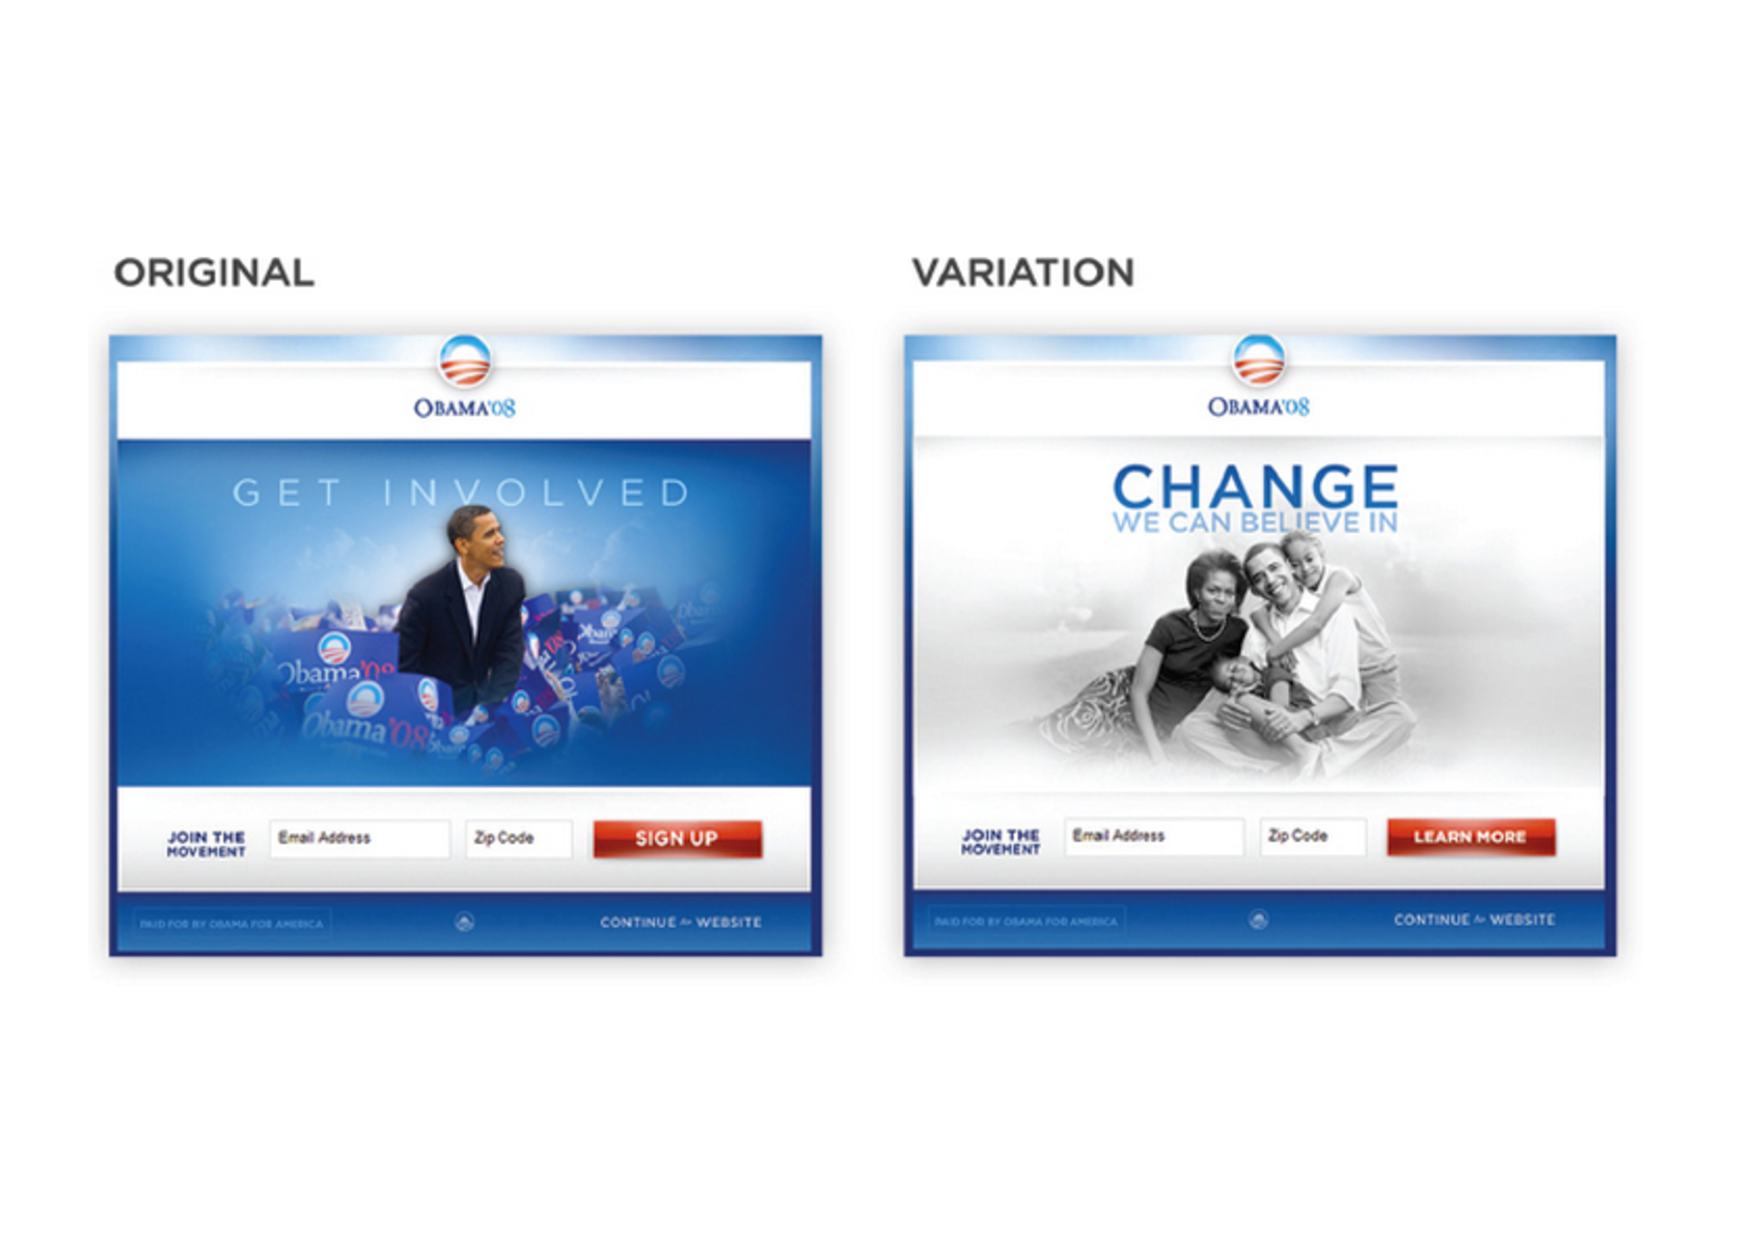
\includegraphics[height=10cm]{diagrams/obama2008}
\caption{Two competing designs from the Obama 2008 presidential campaign \cite[Fig. 1.3]{Siroker2013}\label{obama}}
\end{figure}

Four years later in 2012, the Barak Obama campaign raised over \$1 billion \cite{Ashkenas2012}. A year later, the Finnish mobile game company Supercell made \$892 million of revenue in 2013 with 138 employees leaves little to debate\cite{forbes-supercell}.

Were the Obama fundraising staff and Supercell game development teams talented? Yes. Were they data driven? Most definitely. Use of controlled experiments to fine tune conversion. The controlled experiment gives a flexible way of trying out several designs head to head to make decisions which improve for example conversion \cite{Siroker2013}.

Businesses such as Netflix \cite{Liu2014}, Amazon \cite[p. 147]{Kohavi2009}, Google \cite{wired-abtesting} and others have successfully increased \textit{return on investment} or ROI of their products and services. Instead of trusting the \textit{Hippo} or Highest paid persons' opinion, design choices are made by running experiments, which has taken the freemium business model to new heights.

The freemium business model has roots in the feature limited software model prevalent in the 1980's \cite{Seufert2014}.\textit{Freemium} was coined in 2006 by Jarid Lukin and defined by Venture Capitalist Fred Wilson to describe a model where free leads to maximizing the number of potential players and revenue is generated by selling premium services inside games\cite{Wilson2006}.

In Supercell's \textit{Hayday} has a price point of \$0. The player can spen money to purchase resources and gain money by selling resources (Figure \ref{hayday-core}).

\begin{figure}[htb]
\centering 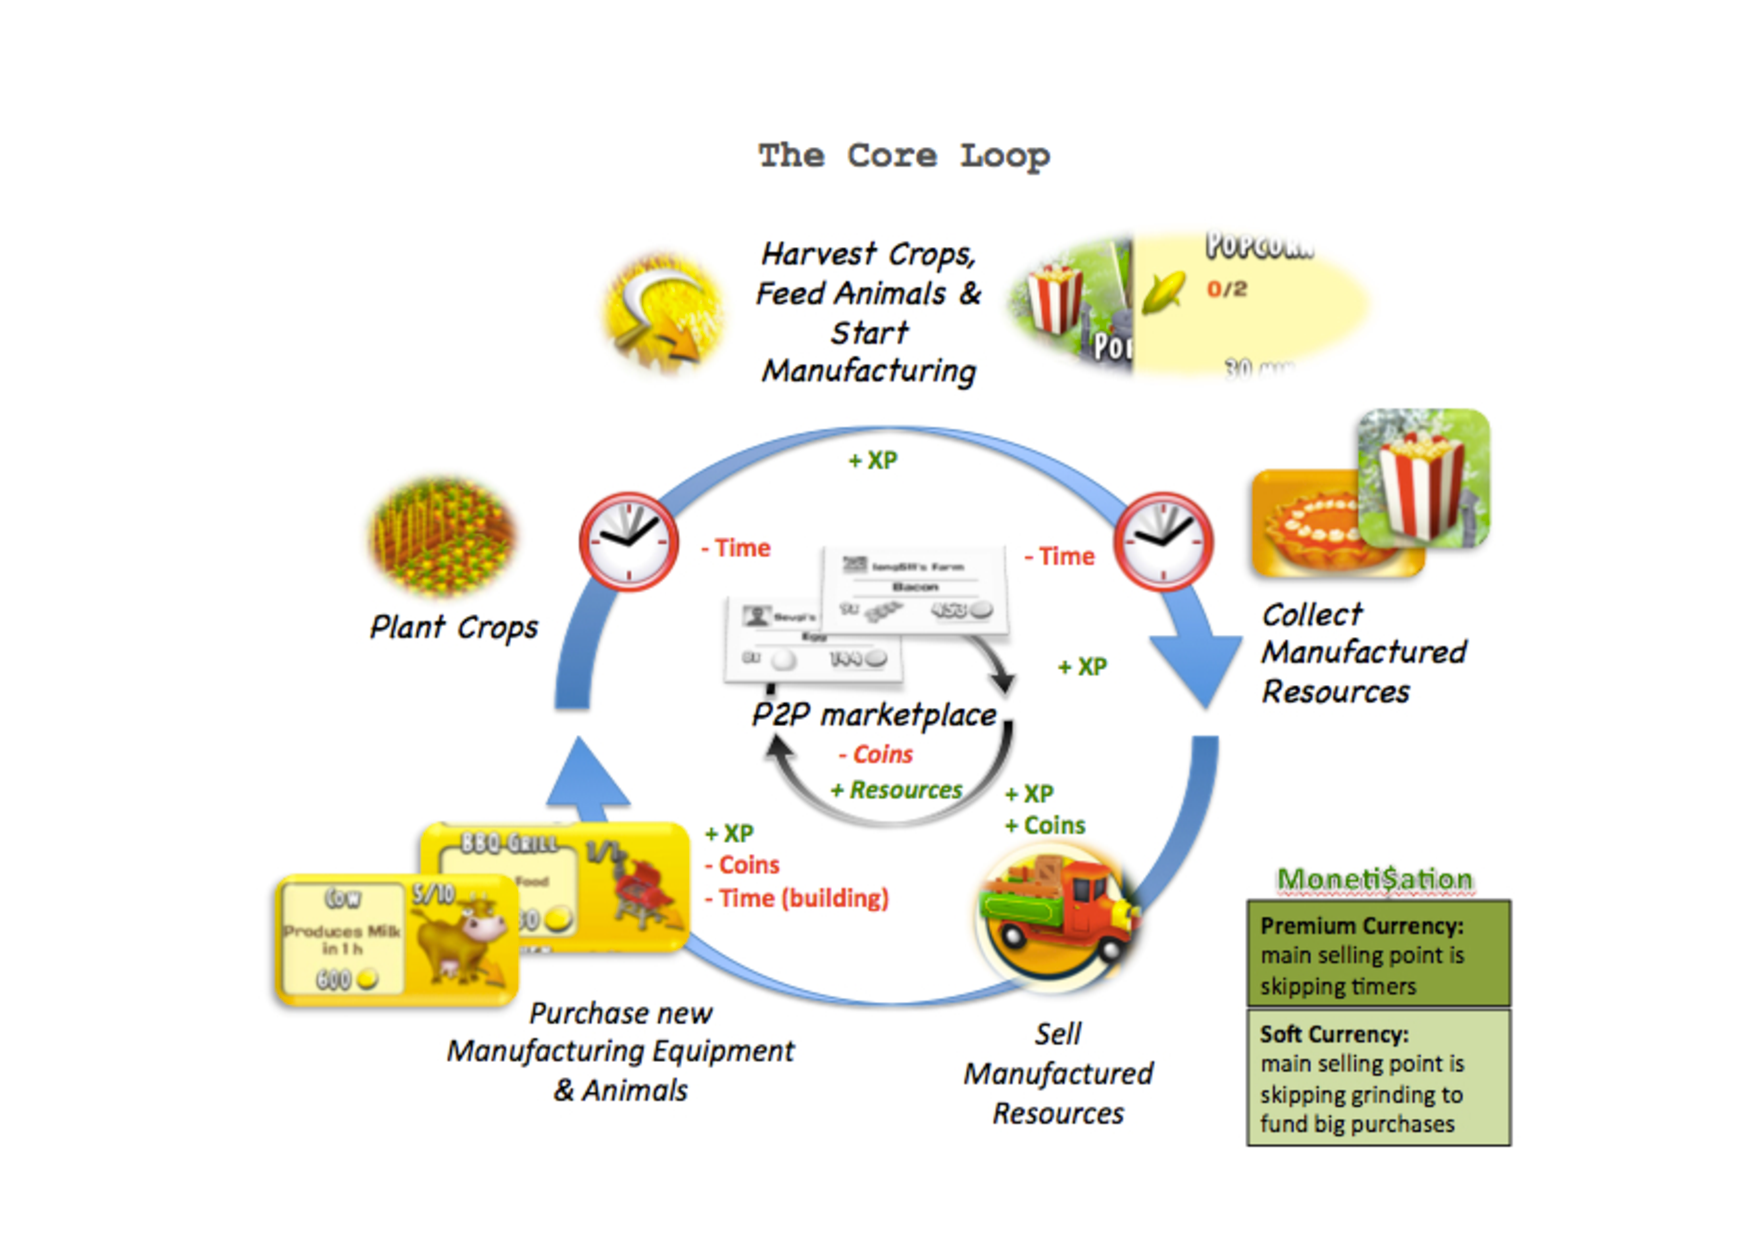
\includegraphics[height=10cm]{diagrams/hayday_core}
\caption{Hay day core loop \cite{Katkoff2013}\label{hayday-core}}
\end{figure}

According to Janne Peltola, a Data Scientist at Supercell ''One interesting A/B test Supercell conducted was about Facebook connectivity. The test was designe to look at whether people who like the games also wanted to encourage their friends to play, and to see how those variables affected player retention.'' At Supercell each team has a data scientist running and analyzing the test results. It takes a well trained professional to gather data, run and analyze the test.\cite{hp-vertica}

The A/B testing process for a single test (Figure \ref{abtesting-steps}) starts with splitting the population who are then exposed to different variations. The user behaviour is then measured and a winner is chosen. If the winner is the control group, no immediate action is taken. If the winner is the variant, the variant is deployed to all users. \cite{Collins2014}

\begin{figure}[htb]
\centering 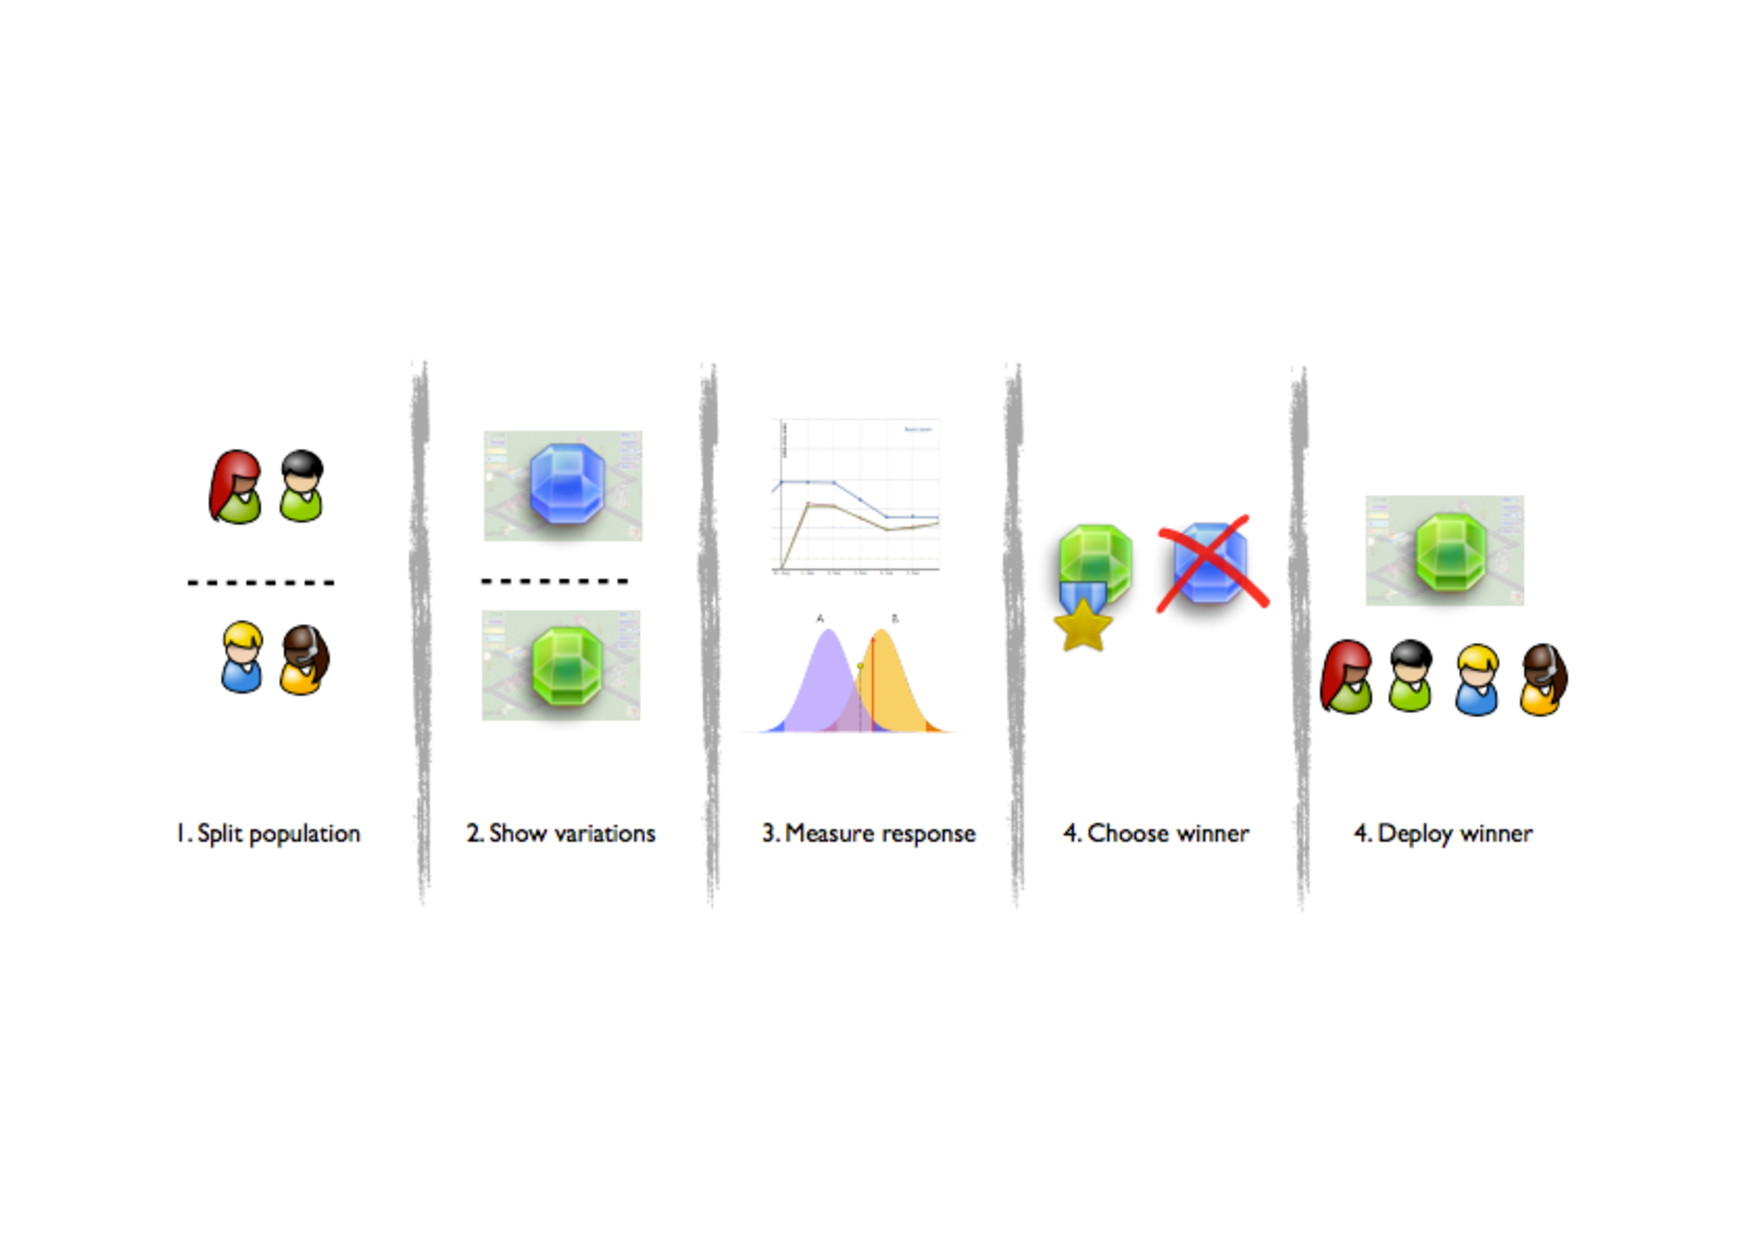
\includegraphics[height=10cm]{diagrams/abtesting_steps}
\caption{Typical steps of an A/B test \cite[p.11]{Collins2014}.\label{abtesting-steps}}
\end{figure}

Could the A/B testing process be automated by a tool so that the test could be run by the game development team instead of hiring a professional. Who are the users of such systems? What are their demands? What are the best practices for running A/B Tests for optimizing a freemium game experience?

The science behind testing is well know as are the methods of testing games, but can we automate test steps of deploying variants, running test, reaching confidence and deploying the winner to all users? Can a usable A/B testing system for creation of freemium games be created? Can this system be safely be used by non professionals to improve game conversion and retention. Moving from some testing by professionals, to ''Always be Testing'' \cite{Siroker2013} at scale supported by tooling.

The A/B Testing system is a confluence of the game team and their tools; the players and their devices and the environment that they are in. The design science paradigm is a good fit for a method to conduct research for such an A/B testing system. Design science research frames the search (Figure \ref{ds}) for such an artifact to implementation and evaluation \cite[p. 75]{Hevner2004}.

Background and theory of controlled experiments will be done first, as well as an introduction to design-science research. The design process will start with analysis of existing A/B testing systems. Initial design with paper prototypes of a user interface for A/B testing which is then rapidly developed to a working prototype with AngularJS. The backend solution will be prototyped using \textit{Hapi.js}. It will not be suitable for large traffic volumes. The system will then be used in the development of a simple game and feedback will be gathered from pilot users. The system will go through a last iteration to accommodate for user feedback and results will be reported.

\clearpage

\section{Methods}
The freemium business model is viable like never before by a confluence of circumstances. Application stores for platforms such as Apples \textit{iOS} (75 billion downloads from the App Store by September 2014 \cite{Perez2014}) and Googles \textit{Android} (50 billion downloads from Google Play \cite{Victor2013}) have made it possible to reach global markets instantly with a marginal cost of production. This combined with price point \$0 allows for massive scale as inhibitors for easy access are removed. In that massive scale one will find the players who are willing to pay for premium services within the game or service.\cite{Seufert2013} In order to reach those willing to pay more for the product than if it was a premium game, the experience needs to be built from the ground up to be freemium. It cannot be added on later, and it is a function of skills. Do you have a team that is able to deliver?\cite{Seufert2013} If the decision is made to go freemium, insight into user behavior in the game context is cardinal. A part of this insight is studying collected user data. Experimentation is a big part of making game design decisions.

A simple A/B test consists of the control group and the variant, which are exposed to different set of users from the pool of all users. The goal is to improve retention and or conversion amongst many others. The expriment is quite similar to clinical trials, where the goal may be to measure the effectiveness of a treatment for example. The roots of the controlled experiment

The Persian philosopher Avicenna gave advice similar to a clinical trial in \textit{The Canon of Medicine} in 1025. In 1601 Sir Richard Lancaster aboard the Red Dragon rationed lemon juice to his crew. On other ships of the fleet where lemon juice was not administered many fell ill with scurvy. The practice lost favor to other less effective treatments. James Lind, a Scotsman ran a controlled experiment in 1747 to determine effects of citrus fruit on patients with scurvy. He gathered evidence to prove treatment of scurvy by citrus fruit effective.\cite{Mellick2009}

Like selecting a treatment for scurvy, perfecting a game design through experimentation is commonplace. Uncertainty comes from the many caveats ahead in applying controlled experiments to game design.

\subsection{Scientific Method}
To improve a game based on solid reasoning, the scientific method is a good guideline. A question is asked and after background research, a hypothesis is formulated. In order to prove or disprove the hypothesis, an experiment is designed and performed. The data collection must be done in a reproducible manner. After results are reported, the study goes through peer review.\cite[p. 224]{Crawford1990}

\begin{figure}[htb]
\centering 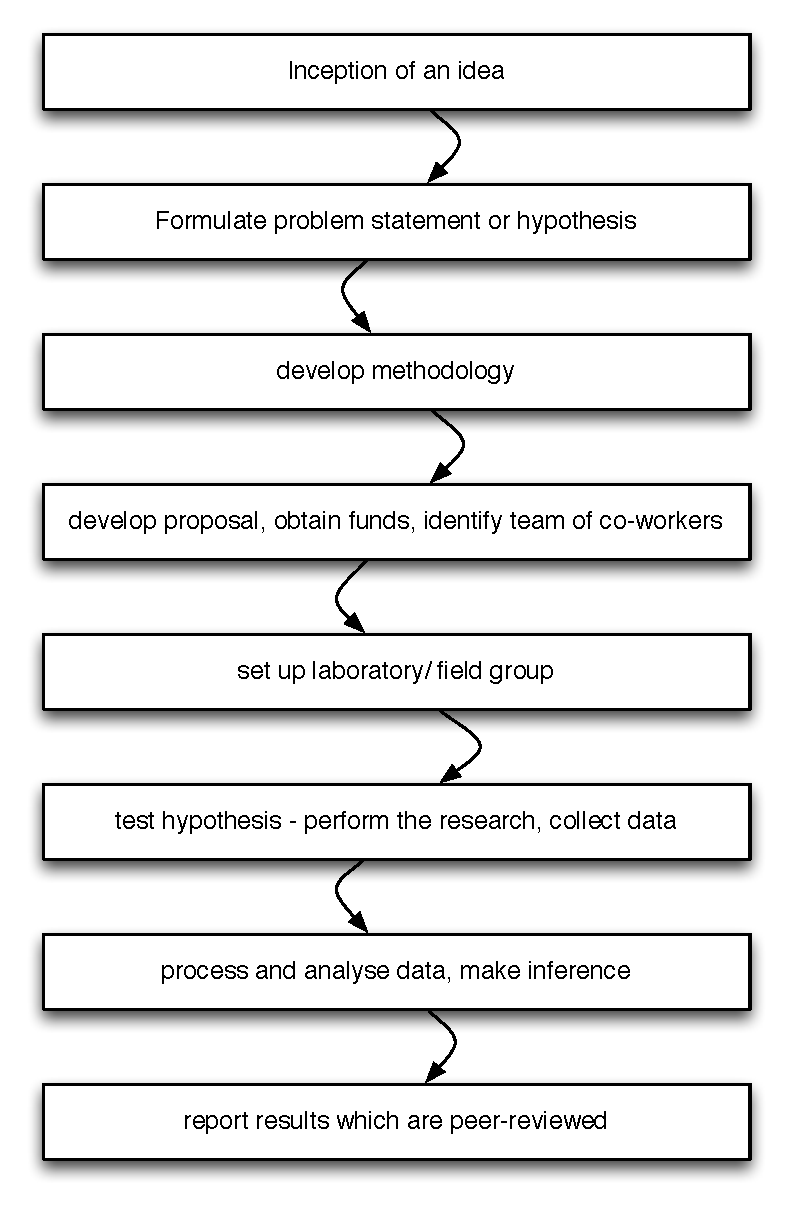
\includegraphics[height=10cm]{diagrams/research_sequence_Crawford1990}
\caption{Sequence of events in a research project \cite[p. 224]{Crawford1990}\label{research}}
\end{figure}

When trying to improve design of a game, asking the question that needs to be answered is vital, because it brings focus to the rest of the process, just like when the scientific method is applied elsewhere. The question is then answered through experimentation.

\subsection{Common Metrics}
With an ideal testing system the team can measure almost any player action.
\subsubsection{Conversion}

\subsubsection{Retention}
\subsubsection{Funnels}
First Time Flow
\subsubsection{Growth}
The net promoter score or \textit{NPS} measures loyalty in customer relationships. The user, player or customer is asked one question ''How likely is it that you would recommend our company/product/service to a friend or colleague?'' The scale could be 0 to 10 for example. \cite{Reichheld2003}

Social graphs like \textit{facebook} allow players to connect via social networks. Virality measures how much your player base grows through viral connections. If 100 players install the game on a given day, and they bring in 10 additional players through social networks, virality is 10\% for that day.\cite{Oracle2012}

\subsection{Controlled Experiment}
The A/B Test, a simple controlled experiment exposes two different versions of the game, or parts of the game to different players. The intent usually is to improve conversion or retention, but these are other goals. The control group represents current game design. The variant is a game design variation. The control and the variant are exposed to different sets of players and player behaviour is observed and analyzed.\cite{}

A ratio of users who converted over total users in a test group is common when comparing test results between control and variant.

\subsubsection{Unbiased Estimate for Ratio}
Choosing $n$ players at random from which the observed number of players who did a desired action is $x$ result in ratio of $p$, which is usually binomially distributed $X ~ Bin(n,p)$. Because $E[X] = np$ the unbiased estimator for $p$ is $p^*=\frac{X}{n}$ and estimate $\hat{p}=\frac{x}{n}$. Here $X$ is a random variable representing the number of players who did desired action.\cite[p.162]{Laininen1998}

\subsubsection{z-Test}
\subsubsection{t-Test}
\subsubsection{Bayesian Approach}
\subsubsection{Multivariate Tests}
\subsubsection{Multiarmed Bandit}
\subsubsection{Confidence Intervals}
\subsubsection{Sample Size}
\subsubsection{Statistical Significance}
\subsubsection{Error}
There are tree ways to arrive at false conclusions in the scientific method; mistakes where there was no way to know that conclusions were incorrect, errors due to negligence, and fraud \cite{Crawford1990}.
\subsubsection{Common mistakes}
Local maxima
Peeking

\subsection{Example cases for A/B Testing}


\subsection{Design-Science Research}
\begin{table}[htb]
\caption{Design Science Research Guidelines \cite[p. 83]{Hevner2004}\label{taulukko1}}
\begin{center}
\fbox{
\begin{tabular}{p{3cm}|p{8cm}}
Design as an Artifact & Design-science research must produce a viable artifact in the form of a construct, a model, amethod, or an instantiation. \\ \hline
Problem Relevance & The objective of design-science research is to develop technology-based solutions to important and relevant business problems.\\ \hline
Design Evaluation & The utility, quality, and efficacy of a design artifact must be rigorously demonstrated via well-executed evaluation methods. \\ \hline
Research Contributions & Effective design-science research must provide clear and verifiable contributions in the areas of the design artifact, design foundations, and or design methodologies. \\ \hline
Research Rigor & Design-science research relies upon the application of rigorous methods in both the construction and evaluation of the design artifact. \\ \hline
Design as a Search Process & The search for an effective artifact requires utilizing available means to reach desired ends while satisfying laws in the problem environment. \\ \hline
Communication of Research & Design-science research must be presented effectively both to technology-oriented as well as management-oriented audiences.
\end{tabular}
}
\end{center}
\end{table}

\subsection{Freemium}


\subsubsection{}

\subsection{Prototyping}
AngularJS for fast prototyping


\subsection{Prior art}
\subsubsection{Amazon A/B Testing (Beta)}
\subsubsection{Splitforce.com}
\subsubsection{Mixpanel}
\subsubsection{GameAnalytics}
\subsubsection{LeanPlum}
\subsubsection{Google Analytics}
\subsubsection{Taplytics}
\subsubsection{AppIterate}

\subsection{Plan}
Prior art. Create first version of front end. Create business logic and domain model. Collect feedback.




%% Osan hienojaottelua alaosiin, eik\"a v\"altt\"am\"att\"a edes tarpeen,
%% t\"ass\"a vain esimerkkin\"a. K\"ayt\"a harkintasi mukaan
%% osan jaottelua, joskus alaotsikot selvent\"av\"at asioita ja
%% joskus vain sirpaloittavat tarpeettomasti teksti\"a.
%%  Jaottelu menee seuraavasti:
%% \section{osan otsikko}
%% \subsection{alaotsikko}
%% \subsubsection{ala-alaotsikko}
%% T\"at\"a pitem\"alle ei pid\"a jaotella.
%%
%% Three levels of hierarchy in sectioning should be enough

\subsection*{Rakenne}

Opinn\"aytteen rakenteen tulee olla hyv\"an tieteellisen
kirjoittamisen k\"ayt\"ann\"on mukainen ja sis\"alt\"a\"a v\"ahint\"a\"an seuraavat
osat:

\begin{enumerate}
\item Nimi\"olehti
\item Tiivistelm\"a
\item Sis\"allysluettelo
\item Symboli- ja lyhenneluettelo
\item \label{a} Johdanto
%% T\"ass\"a alla on esimerkki lainausmerkkien k\"ayt\"ost\"a. Suomalaisen tekstin
%% lainausmerkit eiv\"at mene oikein latexissa (tai monissa muissakaan
%% julkaisuj\"arjestelmiss\"a) kun k\"aytet\"a\"an
%% "-merkki\"a, koska latex k\"aytt\"a\"a amerikkalaista lainausmerkkien
%% tulostustapaa. Vaihtoehtona voi k\"aytt\"a\"a kulmalainausmerkkej\"a, jotka
%% my\"os tulostuvat oikein.
\item  Aikaisempi tutkimus. Ty\"on luonteen niin vaatiessa otsikko voi olla my\"os
        >>Teoreettinen tausta>>  tai n\"aiden otsikoiden yhdistelm\"a.
\item Tutkimusaineisto ja -menetelm\"at %% yhdysmerkki - eli tavuviiva.
\item Tulokset
\item \label{o} Tarkastelu. Ty\"on luonteen niin vaatiessa otsikko voi
      olla my\"os >>Johtop\"a\"at\"okset>> tai >>Yhteenveto>>
      tai edell\"a mainittujen otsikoiden yhdistelm\"a.
\item L\"ahteet
\item Liitteet.
\end{enumerate}

Tiivistelm\"an ja symboli- sek\"a lyhenneluetteloiden
v\"aliin voi sijoittaa halutessaan esipuheen.

Ty\"on osat \ref{a}-\ref{o} muodostavat \textit{tekstiosan.}  Ty\"on
yksitt\"aisi\"a osia voidaan jakaa alaotsikoilla alaosiin, joita ei ole
yll\"a esitetty. Alaotsikoiden k\"aytt\"aminen selvent\"a\"a parhaimmillaan
teksti\"a, ja pahimmillaan sirpaloittaa sit\"a.  Sirpaloitumista voi est\"a\"a
huolehtimalla siit\"a, ett\"a samalla sivulla ei esiinny useampaa
alaotsikkoa.  Tekstin j\"asentelyss\"a on yleens\"a ongelmia, jos osassa on
vain yksi alaosa, tai kirjoittaja joutuu k\"aytt\"am\"a\"an useampaa kuin
kahta tasoa (osa ja alaosat): alaosien alaosat ovat harvoin tarpeen.
\subsection*{Sivut ja kirjaintyypit}

Opinn\"aytteen tulee olla kirjoitettu koneella tai
tekstink\"asittelyohjelmalla yksipuolisesti A4-kokoiselle paperille.
Kandidaatinty\"on tekstiosan sopiva pituus on noin 15--20 sivua ja
diplomity\"on noin 60 sivua. Ty\"ot\"a ei ole syyt\"a tarpeettomasti pident\"a\"a.

Opinn\"aytteen tekstiosan kirjaintyypin tulee olla antiikva eli
%% esimerkki pakkotavutuksesta; "serif-tyyppinen" on tavutuksen kannalta
%% hankala, joten pakkotavutetaan se.
serif\--tyyp\-pi\-nen ja lis\"aksi kursivoimaton, lihavoimaton sek\"a kooltaan 12
pistett\"a (kuten t\"ass\"a esityksess\"a). Groteskeja eli \textsf{Sans
  serif}-tyyppisi\"a kirjaintyyppej\"a (kuten Helvetica tai Arial) ei saa
k\"aytt\"a\"a varsinaisessa tekstiss\"a, mutta otsikoissa n\"ait\"a voidaan
k\"aytt\"a\"a.  Otsikoissa voidaan k\"aytt\"a\"a kooltaan edell\"a mainittua
suurempaa kirjaintyyppi\"a sek\"a tyylikeinoja, kuten lihavointia tai
kursivointia.  Tekstiss\"a samantasoisten otsikoiden on kuitenkin oltava
tyylilt\"a\"an ja kirjainlajeiltaan yhtenev\"aisi\"a.
%% Esimerkki taulukosta
\begin{table}[htb]
%% Taulukon teksti
\caption{Taulukoissa ja kuvissa kirjaintyypin voi valita
tarkoituksenmukaisesti, mutta kuva- ja taulukkoteksteiss\"a tulee
k\"aytt\"a\"a samaa kirjaintyyppi\"a kuin varsinaisessa tekstiss\"a.
Huomaa taulukon numeroinnin sijoittuminen taulukon yl\"apuolelle. \label{taulukko1}}
\begin{center}
\fbox{
\begin{tabular}{c|l|r}
\textbf{A} & 1 & $e^{j \omega t}$ \\ \hline
\textsf{B} & 2 & ${\mathfrak R}(c)$ \\ \hline
\texttt{C} & 3 & $ a \in \mathbb{A}$
\end{tabular}
}
\end{center}
\end{table}

Opinn\"aytteen vasen marginaali (sidonnan puoli) on
35~mm % t\"ass\"a ~ muodostaa ns. yhdist\"av\"an v\"alily\"onnin
ja oikea 25~mm. Yl\"amarginaali on 25~mm. Leip\"atekstin korkeus on
enimmill\"a\"an 230mm. T\"am\"an opinn\"aytepohjan marginaalien pit\"aisi olla
paperille tulostettuna oikein, mutta tulostimesta ja paperista
riippuen voi esiinty\"a yhden tai kahden millimetrin suuruisia eroja.
%% Jos k\"a\"ann\"at t\"am\"an tekstin pdflatex-komennolla ja tulostat sen katselu-
%% ohjelmasta, toteat todenn\"ak\"oisesti em. mittojen poikkeavan enemm\"an
%% kuin 1-2 mm.
%% T\"am\"a on seurausta pdf-tiedoston erilaisesta kirjaintyyppim\"a\"arityksest\"a.
%% Korkeatasoista painoty\"ot\"a varten k\"ayt\"a vain latex-komentoa ja
%% tulosta postscript-muotoon k\"a\"annetyst\"a tiedostosta.
\subsection*{Asemointi}

%% Muutos vanhaan ohjeeseen verrattuna: aikaisemmassa ohjeessa
%% kehotettiin k\"aytt\"am\"a\"an vasensuora-asettelua, mutta t\"ass\"a
%% ohjeessa ollaan luovuttu tuosta vaatimuksesta ja siirrytty
%% huoliteltumpaan, painotuotteenomaisempaan suuntaan.
Tekstiosan tekstiss\"a k\"aytet\"a\"an kappaleiden erottamiseen sisennyst\"a,
mutta ensimm\"aist\"a otsikon, v\"aliotsikon tai muun katkon j\"alkeist\"a
kappaletta ei sisennet\"a. Jos kuva tai muu katko tulee kappaleiden
v\"aliin, suositellaan katkon j\"alkeisen kappaleen sisent\"amist\"a.

Mik\"ali oikea reuna halutaan tasata, tulee k\"aytt\"a\"a tavutusta ja lis\"aksi
tarkistaa, ettei tekstiin j\"a\"a lukemista h\"airitsevi\"a pitki\"a sanav\"alej\"a. Jos
k\"ayt\"at opinn\"aytteen tekemisess\"a \LaTeX-j\"arjestelm\"a\"a,
t\"am\"a asia hoituu automaattisest.

Opinn\"aytteen riviv\"ali on 1, mik\"a on my\"os t\"am\"an opinn\"aytepohjan k\"ayt\"ant\"o.
Kappaleiden tulee yleens\"a olla ainakin kolmen rivin pituisia, mutta
my\"os liian pitki\"a kappaleita tulee v\"altt\"a\"a.  T\"ass\"a opinn\"aytepohjassa
ei tekstin luonteen vuoksi voida t\"aysin toteuttaa kappaleen pituutta koskevia
vaatimuksia.

Yksitt\"aisi\"a, kappaleen p\"a\"att\"avi\"a tai aloittavia rivej\"a sivun alussa
tai lopussa on v\"altett\"av\"a koko ty\"oss\"a, my\"os luetteloissa ja
liitteiss\"a.

\subsection*{Numerointi}

Opinn\"aytteen jokainen osa alkaa uudelta sivulta. Alaosa aloittaa uuden
sivun vain edellisen sivun t\"aytytty\"a.

Ty\"on osat numeroidaan siten, ett\"a johdanto on ensimm\"ainen numeroitava
osa. Osien numeroinnissa k\"aytet\"a\"an arabialaisia numeroita.

Nimi\"olehti, tiivistelm\"a, esipuhe, sis\"allysluettelo ja symboli- ja
lyhenneluettelo numeroidaan esipuheesta tai t\"am\"an puuttuessa
ensimm\"aiselt\"a luettelosivulta alkaen roomalaisin numeroin.

Sivunumerointi alkaa toiselta varsinaiselta tekstisivulta, ja
sivunumeroinnissa k\"aytet\"a\"an arabialaisia numeroita.

L\"ahdeluettelo alkaa uudelta sivulta. L\"ahdeluettelon sivunumerointi
jatkuu viimeisest\"a tekstisivusta.

Jokainen liite alkaa uudelta sivulta. Liitteiden sivunumerointi
jatkuu viimeisest\"a l\"ahdeluettelon sivusta.

Sivunumero sijoitetaan sivun yl\"areunaan.

Matemaattiset kaavat numeroidaan arabialaisin
numeroin. Kaavanumerointi ei saa katketa osien v\"aliss\"a (eik\"a niin
tapahdukaan, jos k\"ayt\"at t\"at\"a opinn\"aytepohjaa). Kaikkia kaavoja ei tarvitse
numeroida, vaan kirjoittaja voi k\"aytt\"a\"a harkintaa numeroinnin
tarpeellisuudessa.  Liitteiss\"a olevat kaavat numeroidaan siten, ett\"a
liitteen ajatellaan muodostavan numeroinnin kannalta itsen\"aisen ja
yhten\"aisen kokonaisuuden. Kaavan numero sijoitetaan oikealle puolelle
alla olevan esimerkin mukaisesti
\begin{equation}
D(xy) = (Dx)y + x(Dy),  \hspace{3em} x,y \in \mathbb{A}.
\end{equation}
%% Kaavojen j\"alkeen ei yleens\"a laiteta sisennyst\"a.
Kaikki kuvat ja taulukot numeroidaan erillisen juoksevan numeroinnin
mukaisesti kuten taulukosta \ref{taulukko1} ja kuvasta \ref{kuva1} k\"ay
ilmi.  Liitteiss\"a olevat kuvat ja taulukot numeroidaan siten, ett\"a
liitteen ajatellaan muodostavan numeroinnin kannalta itsen\"aisen ja
yhten\"aisen kokonaisuuden. Liitteiss\"a \ref{LiiteA} ja \ref{LiiteB} on
esimerkkej\"a kaavojen (kaavat \ref{liitekaava1}--\ref{liitekaava2} tai
kaavat \ref{liitekaava3}--\ref{liitekaava4}), kuvien (kuva
\ref{liitekuva}) ja taulukoiden (taulukko \ref{liitetaulukko})
numeroimisesta.  Liitteet numeroidaan suuraakkosin (esimerkiksi Liite
A, Liite B tai pelk\"ast\"a\"an A, B).
%% T\"ass\"a esimerkki kuva1.pdf -nimisen tiedoston tuomisesta kuvaksi.
%% Komento \inclugraphics[parametrit]{argumentti} tuo kuvan.
%% Komento \centering pakottaa kuvan keskelle.
%% Komento \caption luo kuvatekstin ja sen numeroinnin
%% Parametrit htb pakottavat kuvan suunnilleen siihen
%% kohtaan, miss\"a se esiintyy tekstin l\"ahdekoodissa
\begin{figure}[htb]
\centering 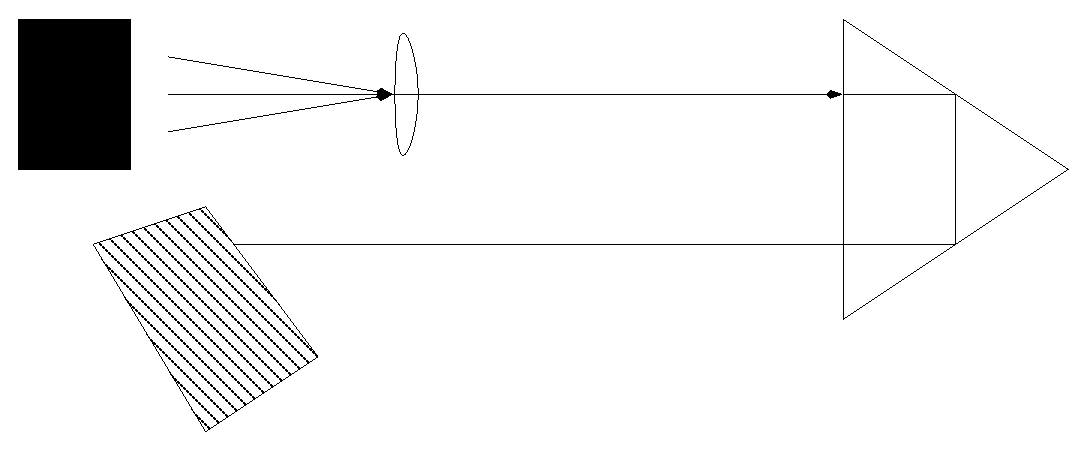
\includegraphics[height=5cm]{kuva1}
\caption{T\"am\"a on esimerkki numeroidusta kuvatekstist\"a. \label{kuva1}}
\end{figure}

\subsection*{L\"ahdeviittausten k\"aytt\"o}

L\"ahdeviittaukset tulee tehd\"a huolellisesti ja johdonmukaisesti
numeroviitej\"arjestelm\"an mukaisesti. Numeroviitteet j\"arjestet\"a\"an
l\"ahdeluetteloon viittausj\"arjestykseen, mutta jos l\"ahdeluettelo
on hyvin laaja (useita sivuja), j\"arjestet\"a\"an viitteet p\"a\"asanan
mukaiseen aakkosj\"arjestykseen. Alaviitej\"arjestelm\"a\"a
\footnote{My\"osk\"a\"an alaviitteen\"a olevia kommentteja \underline{ei} suositella
k\"aytett\"aviksi.} ei k\"aytet\"a.

Viitteen sijoittelussa noudatetaan seuraavia s\"a\"ant\"oj\"a:
Jos viite kohdistuu vain yhteen virkkeeseen tai virkkeen
osaan, viite \cite{Kauranen} sijoitetaan virkkeen sis\"a\"an ennen virkett\"a
p\"a\"att\"av\"a\"a pistett\"a. Jos taas viite koskee tekstin useampaa
virkett\"a tai kokonaista kappaletta, sijoitetaan viite kappaleen loppuun
pisteen j\"alkeen. \cite{Kauranen}

\subsection*{L\"ahdeluettelo}

L\"ahdeluettelossa esiintyy tavallisesti seuraavassa esitett\"avi\"a
l\"ahteit\"a, joista on numeroviitej\"arjestelm\"ass\"a ilmoitettava
asianomaisessa kohdassa vaaditut tiedot.

%% Esimerkki korostamisesta. Lihavoinnin sijasta on tyylikk\"a\"amp\"a\"a
%% ja luettavampaa k\"aytt\"a\"a kursiivia.
\textit{Kirjasta} ilmoitetaan seuraavat tiedot:

\begin{itemize}
\item[--]tekij\"at
\item[--]julkaisun nimi
\item[--]painos, jos useita
\item[--]kustannuspaikka
\item[--]julkaisija tai kustantaja
\item[--]julkaisuaika
\item[--]mahdollinen sarjamerkint\"o.
\end{itemize}

Viitteet \cite{Kauranen}--\cite{Koblitz} ovat esimerkkej\"a kirjan
esitt\"amisest\"a l\"ahdeluettelossa. Viite \cite[s.\ 83--124]{Koblitz} on
esimerkki l\"ahdeluettelossa esiintyv\"an kirjan tiettyjen sivujen
esitt\"amisest\"a tekstiss\"a.

\textit{Artikkelista} kausijulkaisussa ilmoitetaan seuraavat tiedot:

\begin{itemize}

\item[--]tekij\"at
\item[--]artikkelin nimi
\item[--]kausijulkaisun nimi
\item[--]julkaisuvuosi
\item[--]kausijulkaisun volyymi tai ilmestymisvuosi
\item[--]kausijulkaisun numero
\item[--]sivut, joilla artikkeli on.
\end{itemize}

Viitteet \cite{bcs}--\cite{Deschamps} ovat esimerkkej\"a artikkelin
esitt\"amisest\"a l\"ahdeluettelossa.

\textit{Kokoomateoksen luvusta tai osasta} ilmoitetaan seuraavat tiedot:

\begin{itemize}
\item[--]luvun tai osan tekij\"at
\item[--]luvun tai osan nimi
\item[--]maininta >>Teoksessa>>
\item[--]koko teoksen toimittajat sek\"a maininta >>(toim.)>>
\item[--]koko teoksen tai konferenssin nimi
\item[--]konferenssiesitelm\"an kyseess\"a ollessa sen pitopaikka ja -aika
\item[--]painos, jos useita
\item[--]kustannuspaikka
\item[--]julkaisija tai kustantaja, jos aihetta t\"am\"an ilmoittamiseen on
\item[--]julkaisuaika
\item[--]sivut, joilla luku tai osa on
\item[--]mahdollinen sarjamerkint\"a.
\end{itemize}

Viitteet \cite{Sihvola}--\cite{Lindblom} ovat esimerkkej\"a
kokoomateoksen luvun tai osan esitt\"amisest\"a l\"ahdeluettelossa.

\textit{Opinn\"aytety\"ost\"a} ilmoitetaan seuraavat tiedot:

\begin{itemize}
\item[--]tekij\"a
\item[--]ty\"on nimi
\item[--]opinn\"aytety\"on tyyppi
\item[--]oppilaitoksen nimi
\item[--]osaston, laitoksen tai ohjelman nimi
\item[--]oppilaitoksen sijaintipaikka
\item[--]vuosiluku.
\end{itemize}

Viitteet \cite{Miinusmaa}--\cite{Lonnqvist} ovat esimerkkej\"a
opinn\"aytteen esitt\"amisest\"a l\"ahdeluettelossa.

\textit{Standardista} ilmoitetaan seuraavat tiedot:

\begin{itemize}
\item[--]standardin tunnus ja numero
\item[--]standardin nimi
\item[--]painos, mik\"ali ei ole ensimm\"ainen
\item[--]julkaisupaikka
\item[--]julkaisija
\item[--]julkaisuvuosi
\item[--]sivum\"a\"ar\"a.
\end{itemize}
Viite \cite{sfs} on esimerkki standardin esitt\"amisest\"a opinn\"aytteen
l\"ahdeluettelossa.

\textit{Haastattelusta} ilmoitetaan seuraavat tiedot:

\begin{itemize}
\item[--]haastatellun henkil\"on nimi
\item[--]haastatellun henkil\"on arvo tai asema
\item[--]haastatellun henkil\"on edustama organisaatio
\item[--]organisaation osoite
\item[--]maininta siit\"a, ett\"a kyseess\"a on haastattelu ja haastattelun
p\"aiv\"am\"a\"ar\"a.
\end{itemize}

Viite \cite{haastattelu} on esimerkki
haastattelun esitt\"amisest\"a l\"ahdeluettelossa.

Osa s\"ahk\"oisess\"a muodossa olevista artikkeleista on saatavissa my\"os
painettuina. \textit{Vain verkosta saatavissa olevasta artikkelista} esitet\"a\"an
seuraavat tiedot:

\begin{itemize}
\item[--]tekij\"at
\item[--]artikkelin nimi
\item[--]kausijulkaisun nimi
\item[--]viestintyyppi
\item[--]laitos tai volyymi
\item[--]kausijulkaisun yksitt\"aist\"a osaa koskeva merkint\"a tai numero
\item[--]julkaisuvuosi tai maininta >>P\"aivitetty>> ja p\"aivitysaika
\item[--]maininta >>Viitattu>> ja viittaamisen ajankohta
\item[--]maininta >>Saatavissa>> ja URL tai
        maininta >>DOI>> ja DOI-numero (DOI=Digital Object Identifier).
\end{itemize}

Viitteet \cite{Ribeiro}--\cite{kone} ovat esimerkkej\"a s\"ahk\"oisess\"a
muodossa olevan artikkelin esitt\"amisest\"a opinn\"aytteen
l\"ahdeluettelossa.  Viitteet \cite{Ribeiro} ja \cite{Stieber} ovat
saatavissa sek\"a painettuna ett\"a verkosta, joten viitteiden esitystapa
mukailee painetun artikkelin viitteen esitystapaa, mutta sen lis\"aksi
kerrotaan julkaisun olevan verkkolehti ja lehden olevan saatavissa
my\"os painettuna.  Viite \cite{kone} on saatavissa vain verkosta ja
siit\"a esitet\"a\"an yll\"a vaaditut tiedot.

Valitettavasti s\"ahk\"oisess\"a muodosssa olevasta artikkelista ei ole aina
saatavissa lai\-tos-, volyymi- tai numerotietoja.

\textit{S\"ahk\"oisess\"a muodossa olevasta opinn\"aytety\"ost\"a} ilmoitetaan
seuraavat tiedot:

\begin{itemize}
\item[--]tekij\"a
\item[--]ty\"on nimi
\item[--]viestintyyppi
\item[--]opinn\"aytety\"on tyyppi
\item[--]oppilaitoksen nimi
\item[--]osaston, laitoksen tai ohjelman nimi
\item[--]oppilaitoksen sijaintipaikka
\item[--]vuosiluku
\item[--]viittamisen ajankohta
\item[--]maininta >>Saatavissa>> ja URL tai
        maininta >>DOI>> ja DOI-numero.
\end{itemize}

Viite \cite{Adida} on esimerkki s\"ahk\"oisess\"a muodossa olevan
opinn\"aytteen esitt\"amisest\"a l\"ahdeluettelossa.

Viite \cite{viittaaminen} on esimerkki itsen\"aisen kirjoituksen sis\"alt\"av\"ast\"a
verkkosivusta. T\"allainen l\"ahde on rinnastettavissa erillisteokseen.
\textit{Verkkosivusta} esitet\"a\"an tiedot:

\begin{itemize}
\item[--] tekij\"at
\item[--] otsikko
\item[--] maininta >>P\"aivitetty>> ja p\"aivitysaika
\item[--] maininta >>Viitattu>> ja viittaamisen ajankohta
\item[--] Maininta >>Saatavissa>> ja URL.
\end{itemize}

Joskus verkkosivun kirjoitus on jaettu useammalle sivulle, jolloin
l\"ahdeluetteloon kirjataan vain sellainen verkko-osoite, joka koskee
koko kirjoitusta tai sen etusivua, ellei sitten
todella tarkoiteta kirjoituksen yksitt\"aist\"a sivua.

\subsection*{Muuta huomioitavaa l\"ahdeluettelossa}

%% Muutos vanhoihin ohjeisiin koskien kielt\"a.
L\"ahdeluettelossa ty\"on ja julkaisun nimi kirjoitetaan alkuper\"aisess\"a
muodossaan. Julkaisijan kotipaikka kirjoitetaan alkukielisess\"a
muodossaan.

Viittamista koskevassa suomalaisessa standardissa
SFS 5342 \cite{sfs} vaaditaan julkaisuista ilmoitettavaksi my\"os ISBN- tai
ISSN-numerot, mutta n\"aiss\"a opinn\"ayteohjeissa ei ISBN- ja
ISSN-numeroita vaadita.

\clearpage

\section{Results}

T\"ass\"a osassa esitet\"a\"an tulokset ja vastataan tutkielman alussa
esitettyihin tutkimuskysymyksiin. Tieteellisen kirjoitelman
arvo mitataan t\"ass\"a osassa esitettyjen tulosten perusteella.

%% Huomaa seuraavassa kappaleessa lainausmerkkien ulkopuolella piste,
%% koska piste ei lopeta lainattua tekstinp\"atk\"a\"a.
%% Jos lainattu tekstinp\"atk\"a loppuu v\"alimerkkiin, tulee v\"alimerkki
%% lainausmerkkien sis\"alle:
%% "Et tu, Brute?" sanoi Caesar kuollessaan.
Tutkimustuloksien merkityst\"a on aina syyt\"a arvioida ja tarkastella
kriittisesti.  Joskus tarkastelu voi olla t\"ass\"a osassa, mutta se
voidaan my\"os j\"att\"a\"a viimeiseen osaan, jolloin viimeisen osan nimeksi
tulee >>Tarkastelu>>. Tutkimustulosten merkityst\"a voi arvioida my\"os
>>Johtop\"a\"at\"okset>>-otsikon alla viimeisess\"a osassa.

T\"ass\"a osassa on syyt\"a my\"os arvioida tutkimustulosten luotettavuutta.
Jos tutkimustulosten merkityst\"a arvioidaan >>Tarkastelu>>-osassa,
voi luotettavuuden arviointi olla my\"os siell\"a.

\clearpage

\section{Discussion}

Discuss finding local maxima and how this is not a replacement for design and talent.

\clearpage

\phantomsection
\addcontentsline{toc}{section}{\refname}
%\addcontentsline{toc}{section}{References}
\bibliographystyle{plain}
\bibliography{abtesting}

\begin{thebibliography}{99}

%% Omat
\bibitem{wired-abtesting} Christian,\ B. The A/B Test: Inside the Technology That’s Changing the Rules of Business,
  \textit{Wired,} magazine, April, 2012.
  Viewed 26.10.2014.  Available:
  \url{http://www.wired.com/2012/04/ff_abtesting/all/}

\bibitem{forbes-supercell} Spence, E. 'Clash of Clans' Developer Supercell Reports \$829 Million In Revenue And A Desire To Support The Finnish Community
\textit{Forbes,} blog, February, 2014.
Viewed 26.10.2014. Available:
\url{http://www.forbes.com/sites/ewanspence/2014/02/12/clash-of-clans-developer-reports-829-million-in-revenue-and-a-desire-to-support-the-finnish-community/}

\bibitem{nielsen2005} Nielsen, J. \textit{Putting A/B Testing in Its Place}, August, 2005.
Viewed 26.10.2014. Available:
\url{http://www.nngroup.com/articles/putting-ab-testing-in-its-place/}

\bibitem{hp-vertica} Hewlett-Packard, \textit{Supercell adopts HP Vertica Analytics Platform,}
February 2014. Available:
\url{http://www.vertica.com/wp-content/uploads/2014/03/SuperCell_Case_Study.pdf}

%% Alla pilkun j\"alkeen on pakotettu oikea v\"ali \<v\"alily\"onti>-merkeill\"a.
\bibitem{Kauranen} Kauranen,\ I., Mustakallio,\ M. ja Palmgren,\ V.
  \textit{Tutkimusraportin kirjoittamisen opas opinn\"aytety\"on
    tekij\"oille.}  Espoo, Teknillinen korkeakoulu, 2006.

\bibitem{Itkonen} Itkonen,\ M. \textit{Typografian k\"asikirja.} 3.\
  painos.  Helsinki, RPS-yhti\"ot, 2007.

\bibitem{Koblitz} Koblitz,\ N. \textit{A Course in Number Theory and
    Cryptography. Graduate Texts in Mathematics 114.}  2.\ painos. New
  York, Springer, 1994.

%% Kun on useampi nimikirjain, jokaisen nimikirjaimen v\"aliin
%% kuuluu v\"alily\"onti. Oikea v\"alin m\"a\"ar\"a on saatu \<v\"alily\"onnill\"a>
\bibitem{bcs} Bardeen,\ J., Cooper,\ L.\ N. ja Schrieffer,\ J.\ R.
  Theory of Superconductivity. \textit{Physical Review,} 1957, vol.\
  108, nro~5, s.\ 1175--1204.

\bibitem{Deschamps} Deschamps,\ G.\ A. Electromagnetics and
  Differential Forms. \textit{Proceedings of the IEEE,} 1981, vol.\
  69, nro~6, s.\ 676--696.

%% Alla esimerkki englanninkielisen tavuttamisen pakottamisesta.
%% Oletusarvoisesti k\"aytet\"a\"an suomalaista tavutusta, mutta viitteiss\"a
%% esiintyy usein muunkielisi\"a lauseita, jotka tulevat siten tavutetuksi
%% suomen kielen s\"a\"ant\"ojen mukaan. T\"am\"an voi korjata \foreignlanguage-
%% komennolla, jonka ensimm\"ainen parametri on vieraan kielen nimi ja toinen
%% on vieraalla kielell\"a tavutettava teksti.
\bibitem{Sihvola} Sihvola,\ A.\ et al.
  \foreignlanguage{english}{Interpretation of measurements of helix
    and bihelix superchiral structures.}
  Teoksessa: Jacob,\ A.\ F. ja
  Reinert,\ J. (toim.) \textit{Bianisotropics '98 7th International
    Conference on Complex Media.}  Braunschweig, 3.--6.6.1998.
  Braunscweig, Technische Universit\"at Braunschweig, 1998, s.\
  317--320.

%% Alla on suomalainen yhdistelm\"asukunimi. Sen nimien v\"aliss\"a
%% k\"aytet\"a\"an yhdysmerkki\"a l. tavuviivaa, kirjoitetaan -.
\bibitem{Lindblom} Lindblom-Yl\"anne,\ S. ja Wager,\ M.  Tieteellisten
  opinn\"aytet\"oiden ohjaaminen. Teoksessa: Lindblom-Yl\"anne,\ S. ja
  Nevgi,\ A. (toim.) \textit{Yliopisto- ja korkeakouluopettajan
    k\"asikirja.}  Helsinki, WSOY, 2004, s.\ 314--325.

\bibitem{Miinusmaa} Miinusmaa,\ H. Neliskulmaisen rei\"an poraamisesta
  kolmikulmaisella poralla. Diplomity\"o, Teknillinen korkeakoulu,
  konetekniikan osasto, Espoo, 1977.

%% T\"ass\"a taas pakotettu englanninkielinen tavutus.
%% Pedanttinen kirjoittaja pakottaa tietysti jokaiseen englanninkieliseen
%% lauseeseen englannin tavutuksen, mutta t\"ass\"a esityksess\"a ei n\"ain ole
%% tehty selvyyden ja l\"ahdekoodin luettavuuden takia.
\bibitem{Loh} Loh,\ N.\ C. High-Resolution Micromachined
  Interferometric Accelerometer. Master's Thesis, Massachusetts
  Institute of Technology, Cambridge,
  \foreignlanguage{english}{Massachusetts,} 1992.

\bibitem{Lonnqvist} L\"onnqvist,\ A.
  \foreignlanguage{english}{Applications of hologram-based compact
    range: antenna radiation pattern, radar cross section, and
    absorber reflectivity measurements.}
  V\"ait\"oskirja, Teknillinen korkeakoulu, s\"ahk\"o- ja tietoliikennetekniikan
  osasto, 2006.

\bibitem{sfs} SFS 5342. Kirjallisuusviitteiden laatiminen. 2.\ painos.
  Helsinki, Suomen standardisoimisliitto, 2004. 20~s.

\bibitem{haastattelu} Palmgren,\ V. Suunnittelija. Teknillinen
  korkeakoulu, kirjasto. Otaniementie 9, 02150 Espoo. Haastattelu
  15.1.2007.

\bibitem{Ribeiro} Ribeiro,\ C.\ B., Ollila,\ E. ja Koivunen,\ V.
  \foreignlanguage{english}{Stochastic Maximum-Likelihood Method for
    MIMO Propagation Parameter Estimation.}
 \textit{IEEE Transactions
    on Signal Processing,} verkkolehti, vol.\ 55, nro~1, s.\ 46--55.
  Viitattu 19.1.2007. Lehti ilmestyy my\"os painettuna. DOI:
  10.1109/TSP.2006.882057.

\bibitem{Stieber} Stieber,\ T. GnuPG Hacks. \textit{Linux Journal,}
  verkkolehti, 2006, maaliskuu, nro~143. Viitattu 19.1.2007. Lehti
  ilmestyy my\"os painettuna. Saatavissa:
  \url{http://www.linuxjournal.com/article/8732.}

\bibitem{kone} Pohjois-Koivisto,\ T. Voiko kone tulevaisuudessa arvata
  tahtosi?  \textit{Apropos,} verkkolehti, helmikuu, nro~1, 2005.
  Viitattu 19.1.2007.  Saatavissa:
  \url{http://www.apropos.fi/1-2005/prima.php.}

\bibitem{Adida} Adida,\ B.  Advances in Cryptographic Voting Systems.
  Verkkodokumentti. Ph.D.\ Thesis, Massachusetts Institute of
  Technology, Cambridge,
  \foreignlanguage{english}{Massachusetts,}
  2006. Viitattu 19.1.2007.  Saatavissa:
  \url{http://crypto.csail.mit.edu/~cis/theses/adida-phd.pdf.}

\bibitem{viittaaminen} Kilpel\"ainen,\ P. WWW-l\"ahteisiin viittaaminen
  tutkielmatekstiss\"a. Verkkodokumentti. P\"aivitetty 26.11.2001.
  Viitattu 19.1.2007. Saatavissa:
  \url{http://www.cs.uku.fi/~kilpelai/wwwlahteet.html.}

\end{thebibliography}

%% Appendices
%% Liitteet
\clearpage

\thesisappendix

\section{Esimerkki liitteest\"a\label{LiiteA}}

Liitteet eiv\"at ole opinn\"aytteen kannalta v\"altt\"am\"att\"omi\"a ja
opinn\"aytteen tekij\"an on
kirjoittamaan ryhtyess\"a\"an hyv\"a ajatella p\"arj\"a\"av\"ans\"a ilman liitteit\"a.
Kokemattomat kirjoittajat, jotka ovat huolissaan
tekstiosan pituudesta, paisuttavat turhan
helposti liitteit\"a pit\"a\"akseen tekstiosan pituuden annetuissa rajoissa.
T\"all\"a tavalla ei synny hyv\"a\"a opinn\"aytett\"a.

Liite on itsen\"ainen kokonaisuus, vaikka se t\"aydent\"a\"akin tekstiosaa.
Liite ei siten ole pelkk\"a listaus, kuva tai taulukko, vaan
liitteess\"a selitet\"a\"an aina sis\"all\"on laatu ja tarkoitus.

Liitteeseen voi laittaa esimerkiksi listauksia. Alla on
listausesimerkki t\"am\"an liitteen luomisesta.

%% Verbatim-ymp\"arist\"o ei muotoile tai tavuta teksti\"a. Fontti on monospace.
%% Verbatim-ymp\"arist\"on sis\"all\"a annettuja komentoja ei LaTeX k\"asittele.
%% Vasta \end{verbatim}-komennon j\"alkeen jatketaan k\"asittely\"a.
\begin{verbatim}
	\clearpage
	\appendix
	\addcontentsline{toc}{section}{Liite A}
	\section*{Liite A}
	...
	\thispagestyle{empty}
	...
	teksti\"a
	...
	\clearpage
\end{verbatim}

Kaavojen numerointi muodostaa liitteiss\"a oman kokonaisuutensa:
\begin{eqnarray}
d \wedge A  &=& F, \label{liitekaava1}\\
d \wedge F  &=& 0. \label{liitekaava2}
\end{eqnarray}


\clearpage
\section{Toinen esimerkki liitteest\"a\label{LiiteB}}

%% Liitteiden kaavat, taulukot ja kuvat numeroidaan omana kokonaisuutenaan
%%
%% Equations, tables and figures have their own numbering in Appendices
%\renewcommand{\theequation}{B\arabic{equation}}
%\setcounter{equation}{0}
%\renewcommand{\thefigure}{B\arabic{figure}}
%\setcounter{figure}{0}
%\renewcommand{\thetable}{B\arabic{table}}
%\setcounter{table}{0}

Liitteiss\"a voi my\"os olla kuvia, jotka
eiv\"at sovi leip\"atekstin joukkoon:
%% Ymp\"arist\"on figure parametrit htb pakottavat
%% kuvan t\"ah\"an, eik\"a LaTeX yrit\"a siirrell\"a niit\"a
%% hyv\"aksi katsomaansa paikkaan.
%% Ymp\"arist\"o\"a center voi k\"aytt\"a\"a \centering-
%% komennon sijaan
%%
%% Example of a figure, note the use of htb parameters which force
%% the figure to be inserted here
\begin{figure}[htb]
\begin{center}
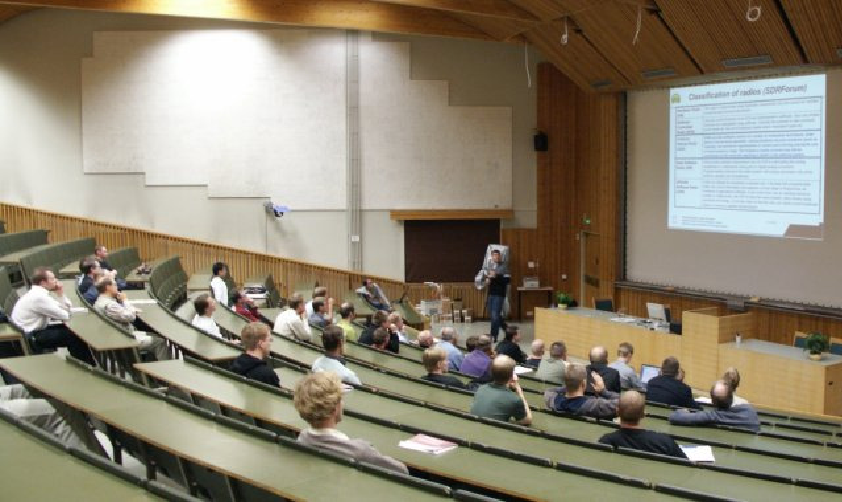
\includegraphics[height=8cm]{kuva2}
\end{center}
\caption{Kuvateksti, jossa on liitteen numerointi}
\label{liitekuva}
\end{figure}
%%
Liitteiden taulukoiden numerointi on kuvien ja kaavojen kaltainen:
\begin{table}[htb]
\caption{Taulukon kuvateksti.}
\label{liitetaulukko}
\begin{center}
\fbox{
\begin{tabular}{lp{0.5\linewidth}}
9.00--9.55  & K\"aytett\"avyystestauksen tiedotustilaisuus (osanottajat
ovat saaneet s\"ahk\"opostitse valmistautumisteht\"av\"at, joten tiedotustilaisuus
voidaan pit\"a\"a lyhyen\"a).\\
9.55--10.00 & Testausalueelle siirtyminen
\end{tabular}}
\end{center}
\end{table}
Kaavojen numerointi muodostaa liitteiss\"a oman kokonaisuutensa:
\begin{eqnarray}
T_{ik} &=& -p g_{ik} + w u_i u_k + \tau_{ik},  \label{liitekaava3} \\
n_i    &=& n u_i + v_i.                      \label{liitekaava4}
\end{eqnarray}

\end{document}
